\documentclass[a4paper,12pt]{article}
\usepackage[T1]{fontenc}
\usepackage[utf8]{inputenc}
\usepackage{lmodern}
\usepackage[french]{babel}
\usepackage{lipsum,url,csquotes}
\usepackage[hidelinks,hyperfootnotes=false]{hyperref}
\usepackage[titlepage,pagenumber]{polytechnique}

\geometry{hmargin=60pt}

\usepackage{amssymb}
\usepackage{babel}
\usepackage{amsmath}
\usepackage{listings}
\usepackage{url}
\usepackage{array}
\usepackage{graphicx}
\usepackage{float}
\usepackage{enumerate}




   \titleformat{\chapter}
        [display]
        {\LARGE\bfseries\sffamily}
        {\LARGE\chaptertitlename{} \thechapter}
        {0em}
        {}
        []
    \titleformat{\section}
        [block]
        {\color{bleu303}\large\bfseries\sffamily\filright}
        {\thesection}{0.6em}
        {\MakeUppercase}
    \titleformat{\subsection}
        [hang]
        {\color{bleu315}\large\scshape}
        {\thesubsection}
        {0.5em}
        {}
     
\titleformat{\subsubsection}
    [block]
    {\color{bleu303}\large\scshape}
    {\thesubsubsection}
    {0.5em}
    {\textbullet{} }
    []
    
    

%----------------------------------------------------------------------------------------
%	TITLE PAGE
%----------------------------------------------------------------------------------------

\title{\vspace{-4em} Euclid vs RSA: Cryptanalysis with batch GCD}
\subtitle{Projet INF442 \#8}

\author{ \large
Diego de Souza | Gabriel Azevedo\\
\vspace{1em}
}

\date{}

\begin{document}

\maketitle
\newpage


\renewcommand*\contentsname{\hfill Sommaire \hfill}

\pagestyle{plain}
\tableofcontents

\newpage

\pagestyle{plain}

\section{Introduction}
RSA is the most widespread public-key cryptosystem on the Internet. Suppose we are given a massive collection of 1024-bit RSA keys. Each of these keys contains a product $N = pq$ of two 512-bit random-looking primes, and the security of the cryptosystem depends on the difficulty of factoring $N$ (that is, deriving $p$ and $q$ given only $N$).
Factoring any one $N$ is a seriously hard problem. But in practice, if we start with a large enough set of
keys, then we can often factor some of them. In an ideal world, no two keys share a $p$ or a $q$. But in
the real world, many keys are generated using poorly-configured (or compromised) random number
generators—which means that occasionally the same prime will pop up in two different keys, and
then we can easily find that common prime as the greatest common divisor (GCD) of the two keys,
using the classic Euclidean algorithm. Computing all of the GCDs pairwise is slow (the difficulty
increases quadratically with the number of keys), but we can do much better using a "batch GCD"
algorithm. The aim of this project is to implement an efficient distributed batch GCD algorithm, and
apply it to collections of millions of RSA keys. The sequential version of this algorithm mirrors a real world attack from 2012, which broke tens of thousands of deployed RSA keys. While
the algorithm appears simple enough, creating a distributed version involves several subtle choices.


\section{Source Code}

\subsection{Organization}
The source code is organized as follows. In the same folder where this report can be found, there is a folder called \textit{source}, as well as a folder called \textit{data}. The folder \textit{data} contains the inputs given by Benjamin Smith. Inside \textit{source} there are two other folders: \textit{sequential}, which contains the code for executing and testing \textit{Task1}, and \textit{distributed}, which contains the software to execute \textit{Task2}.

The code files for each approach are \textit{factors.cpp\/hpp}, \textit{batchGCD.cpp\/hpp} and \textit{main.cpp}. The first one is the class \textit{Factor} for a factorization object (index, first factor p, second factor q), \textit{batchGCD} implements a sequential function to get a vector of \textit{Factor}, and finally the \textit{main} is to test the program. 

\section{Testing the code}
In order to test the code for \textit{Task1} (sequential approach), one can use the following instructions:
\vspace{0.5em}

\lstset{language=Pascal}    

1 - To compile the files:
\begin{lstlisting}[frame=single]
make
\end{lstlisting}

\newline
2 - To use one of the given tests (small and big input):
\begin{lstlisting}[frame=single]
make test_tiny
\end{lstlisting}
or
\begin{lstlisting}[frame=single]
make test_big
\end{lstlisting}
\newline
3- To test a custom input file
\begin{lstlisting}[frame=single]
make
./<executable> <number_of_line_to_be_read> <namefile>
\end{lstlisting}
\newline

where $<executable>$ is the executable file, $<number_of_lines_to_be_read>$ the number of lines to be read and $namefile$ the file's name.


In order to test the code for \textit{Task2} (distributed approach), once the user is inside the \textit{parallel} folder, he can use exactly the same syntax as in the two first previous cases. It works like that because, in the \textit{makefile}, we have preset the number of processors as the following:
\vspace{0.5em}

\lstset{language=Pascal}    
\begin{lstlisting}[frame=single]
NPROC_TINY=20
NPROC_BIG=50
\end{lstlisting}

However, the user can change these values at any time by opening the \textit{makefile} and changing the standart number of processors.

\section{Tasks}
\subsection{Task 0}

\subsubsection{Proving the Batch GDC algorithm}

Proving the Batch GDC algorithm is equivalent to prove that $$gdc(N_i,R_i/N_i) = gdc(N_i,M/N_i)~~~~~~~~[1]$$

where $R_i \equiv M\mod N_i^2$.

Let \textit{l} be the value of the right hand side expression, that is $$l = gdc(N_i,M/N_i)$$

Then, there exist integers $n_i$ and $m_i$ such that
$$N_i = n_i \cdot l ~~~ and~~~ \frac{M}{N_i} = m_i\cdot l ~~~~~ with~~~ gdc(n_i,m_i) = 1$$

From the definition of $R_i$,
$$ \exists k\in \mathbb{N} ~~such~ that~~ 0 \le M - k \cdot N_i^2 < N_i^2 ~~and ~~R_i = M - k \cdot N_i^2$$

Therefore, $R_i$ and $\frac{R_i}{N_i}$ can be rewritten with the following expressions:
$$ R_i = N_i \cdot l\cdot(m_i - k\cdot n_i) ~~~~ and ~~~~\frac{R_i}{N_i} = l(m_i- k\cdot n_i)$$
Replacing this expression on the left hand side of $[1]$, we obtain the following:
$$gdc(N_i,R_i/N_i) = gdc(l\cdot n_i, l\cdot(m_i - k\cdot n_i)) = l\cdot gcd(n_i,m_i-k\cdot n_i))$$

As $gdc(n_i,m_i) = 1$, then $gcd(n_i,m_i-k\cdot n_i)) = 1$. It allows us to conclude that

$$gdc(N_i,R_i/N_i) = l = gdc(N_i,M/N_i)$$

\subsection{Pseudo-code}
It follows a pseudo-code which given a list of $k$ RSA moduli $(N_0, N_1,..., N_k)$, returns a list of known factorizations.


\lstset{language=Pascal}        

\begin{lstlisting}[frame=single]  
Compute product M using a product tree;       Time O(k.M(n))
Compute R intermediate values (R_1,...,R_k);  Time O(k.M(n))

Create a empty list L;

For i from 0 to                       Time O(k.n.M(n))
    Calculate gdc(N_i,R_i/N_i) (p)     
    if p is in [2,N-1] then           
      add(i, p, N_i/p) to L            
\end{lstlisting}


%DIEGO MEXE AQUI EM BAIXO------ completa o TIME na  5a linha de codigo -----------------------DIEGAO
%Compute the product M using a product tree;~~~~   $Time O(k\cdot M(n))$
%
%Compute $R$ intermediate values ($(R_1,...,R_k)$);  ~~~~$Time O(k\cdot M(n))$
%
%Create a empty list L;

%For each $i$ from $0$ to $k$
%~~~~Calculate $gdc(N_i,R_i/N_i)$ ($p$)    $Time O(???)$ 
%~~~~if $p\in [2,N-1]$ then                 $Time O(1)$
%~~~~~~~~add $(i, p, \frac{N_i}{p})$ to L   $Time O(1)$


\subsubsection{Total running time estimation}

As shown in the pseudo-code, the complexity of the algorithm can be expressed as $$O(k\cdot M(n) + k\cdot M(n) + k\cdot n\cdot M(n))$$
Which is equivalent to $$O(k\cdot n \cdot M(n))$$
%----------------------------------------------------------------DIEGO

In order to detail better our reasoning, we can explain each part of the sum: the product takes time $O(M(n))$ for each $N_i$, which gives $O(k\cdot M(n))$. The same reasoning is applied to the calculation of the $R$'s.

Inside the "for" loop there is a $gcd$ calculation, which takes $O(n \cdot M(n))$ in time complexity. With $k$ iterations it gives a total order of $O(k\cdot n \cdot M(n))$ for the loop.
 %------------------------------------------------------------------DIEGO

\subsection{Task 1}
\subsubsection{Implementation}

Our implementation of the Batch GCD's algorithm is structured as follows. It consists basically in a class "BatchGCD", which receives in it's constructor a vector of "mpz\_class" variables and whose function "getFactorization()" returns the factorization vector when called. The vector returned is composed by objects from class "Factor", a class that stores the index of a key and the two factors in which this key can be factorised. The class declarations are shown below.

\lstset{language=C++}        
\begin{lstlisting}[frame=single]
class BatchGCD {
    private:
        //vector of keys
        vector<mpz_class> keys;

        //product tree, initiated in the constructor
        vector< vector<mpz_class> > tree;

    public:
        //fill product tree
        void initTree ();

        //change root value (useful for the distributed algorithm)
        void changeValueRoot(mpz_class x);

        //get root value (useful for the distributed algorithm)
        mpz_class getValueRoot();

        //get remainders to find factors in the batchGCD algorithm
        vector< mpz_class > getRemainders ();

        //c++ wrapper to gcd
        mpz_class gcdCPP (mpz_class p1, mpz_class p2);

        //constructor
        BatchGCD (vector<mpz_class>& keys);

        // factorization of the public keys
        vector<Factor> getFactorization ();

        // print keys
        void printKeys ();
};
\end{lstlisting}


$BatchGDC$'s constructor receives the key inputs and allocate them into the "$keys$" vector. The initTree fill the product tree, which is a vector of vectors of $mpz\_class$ objects.  The $getRemainders$ function traverse the tree and by doing the operation 
$$Current Node = Parent \mod Current Node^2~~~~~~~~~~~~~~~~~~~~[2]$$ 

The $getFactorization$ function calls $getRemainders$ and, then executes the third step of $Batch GDC$'s algorithm: it calculates the $gdc(N_i,R_i/N_i)$ and returns it as a vector of "factor"s objects.

\lstset{language=C++}        
\begin{lstlisting}[frame=single] 
// factorization of the public keys
vector<Factor> BatchGCD::getFactorization () {
    vector <Factor> factors;
    vector<mpz_class> remainders = getRemainders();
    for (long i = 0; i < remainders.size(); i++) {
        mpz_class N = this->keys[i];
        mpz_class p = gcdCPP(N, remainders[i]/N);
        mpz_class q = N/p;
        factors.push_back(Factor(i, p, q));
    }
    return factors;
}

\end{lstlisting}

%----------------------------------------------DIEGO---------------



\subsection{Task 2}

\subsubsection{Implementation}
We decided to split the product tree among the processors, so that each processor only sees and works on a certain branch of the tree. One of the processors, called master, manages and distributes this work.

The algorithm basic structure is described in the pseudo-code below:

%----------precisa de formatar o que vem abaixo
\begin{enumerate}
    \item Master receives the input data
    \item Master distributes the keys among the processors;
   \item Each processor calculates their own and independent product key (sequential batchGCD algorithm);
    \item All processors send their tree's roots to master;
    \item Master uses these roots as keys to build his own product key (that is, applies sequential batchGCD algorithm);
    \item Master uses the operation [2] to create \textit{intermediate Remainders};
    \item \textit{intermediate Remainders} are transmitted to the corresponding processor;
    \item \textit{intermediate Remainders} are then used in each processor as roots to find and print, independently, the list of factors.
\end{enumerate}

Some points deserve deeper explanation in this pseudo-code. The data received is stored in a single array of chars. Each digit (in decimal basis) is expressed by it's correspondent "char", and between two different keys there is always a '\#' (a divisor). An example of the final array is given below.
$$...445522 \# 22255544194155584114242 \# 44229...$$

This array is the one transmitted in step $2$, and the functions used to do so were MPI\_Scatter and MPI\_Scatterv (actually, in order to be able to use the MPI\_Scatter, we have found it necessary to transmit some variables through MPI\_Scatter). The process occurred in the opposite direction in step "$4$" where MPI\_Gather and MPI\_Gatherv functions were used.

The key's distributions (step $2$) can be illustrated as in Figure 1.

	\begin{figure}[H]
		\centering
		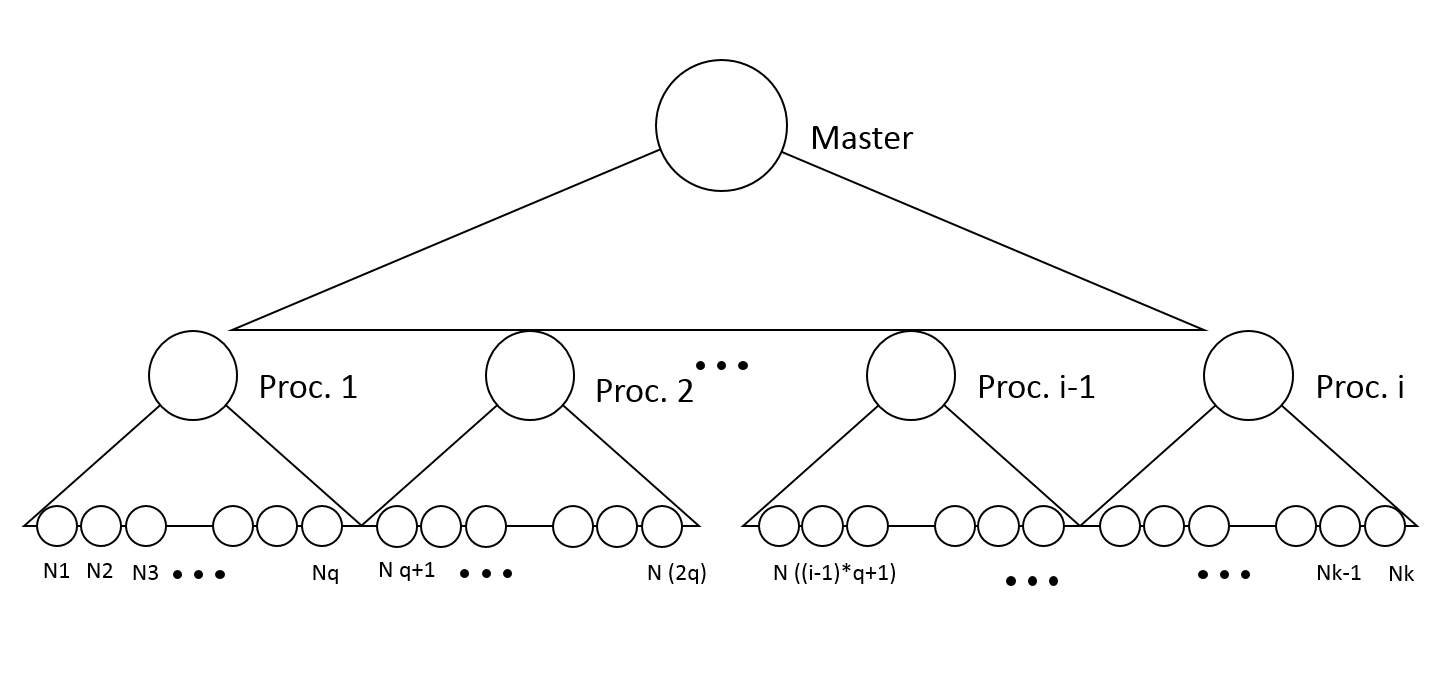
\includegraphics[width=0.65\linewidth]{figure5.png}
		 \caption{Key distributions - step 2}
	\end{figure}

The steps $3$ and $4$ are illustrated in Figure 2. The implementation of $3$ consists in applying Batch GCD's sequential version, discussed previously.

	\begin{figure}[H]
		\centering
		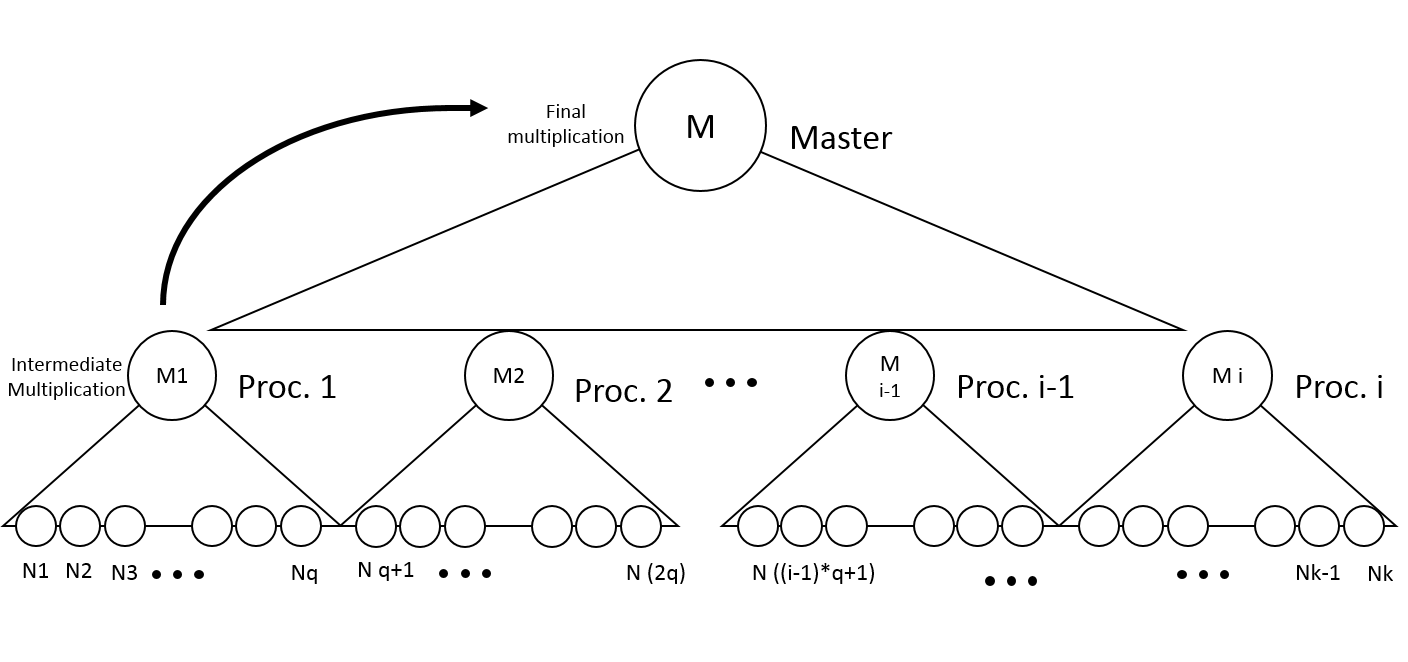
\includegraphics[width=0.65\linewidth]{figure6.png}
		\caption{Constructing product tree - steps 3 and 4}
	\end{figure}

The last 4 steps (5, 6, 7 and 8) are illustrated in Figure 3. 

	\begin{figure}[H]
		\centering
		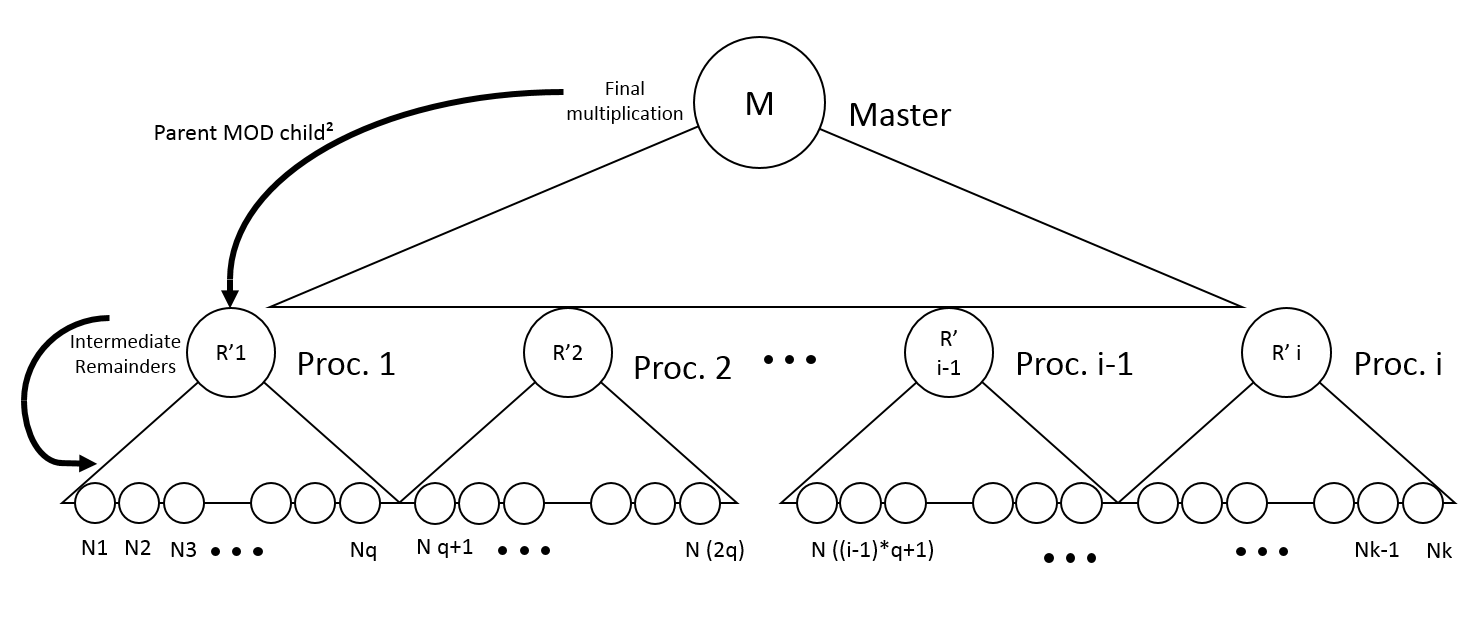
\includegraphics[width=0.65\linewidth]{figure7.png}
		\caption{Finding remainders and printing solution - steps 5, 6, 7 and 8}
	\end{figure}


\subsubsection{Performance}
To visualize how the number of processors affects the performance of the distributed algorithm, the code was executed several times. The results can be found in the following image.

	\begin{figure}[H]
		\centering
		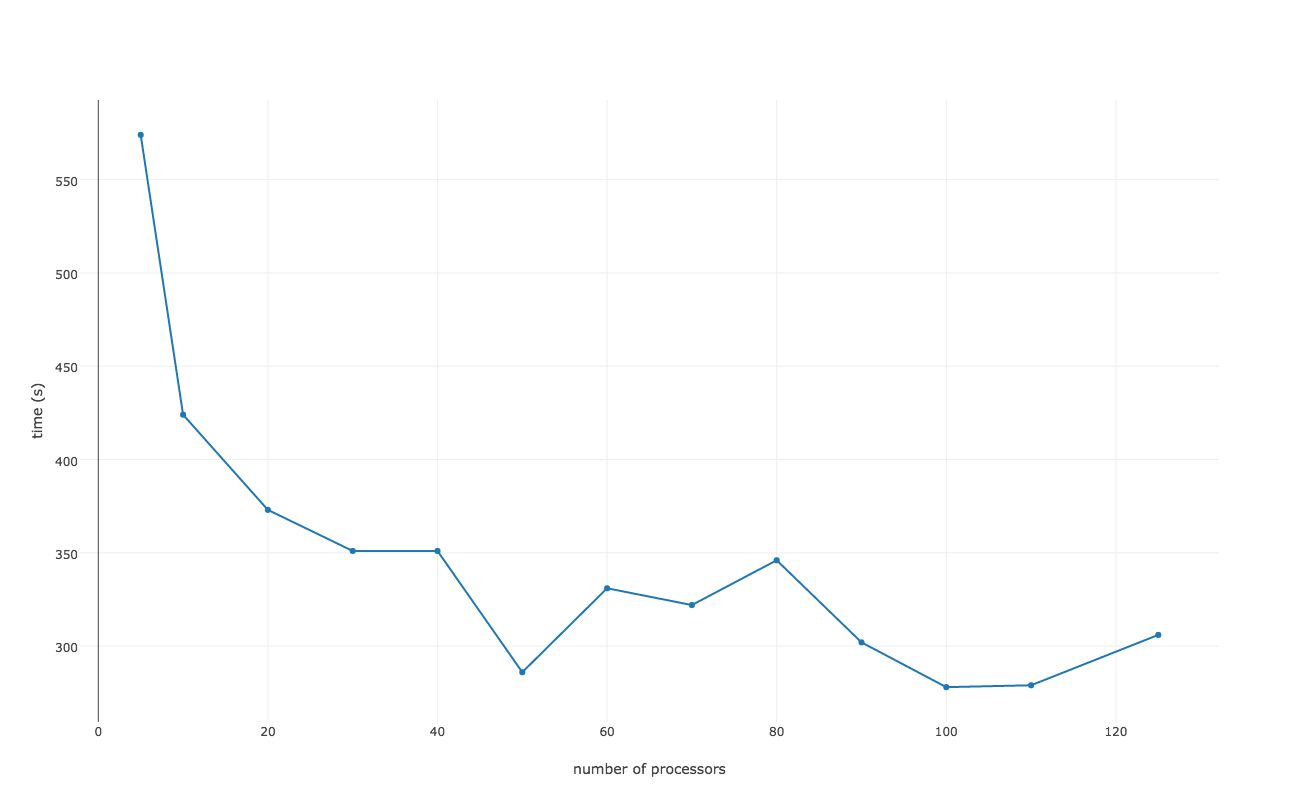
\includegraphics[width=0.9\linewidth]{performance.png}
		\caption{Execution time in function of the number of processors for the bigger input given}
	\end{figure}

It is difficult to measure the execution time with precision, because the machine used can be running many other processes and this affects the execution time. However, based on the graph, the optimal number of processors seems to be 50 or 100 for the bigger given input.

\section{conclusion}
The Batch GCD algorithm has shown satisfactory results in decrypting large numbers by factorisation. In particular, the time execution can be  accelerated by distributing the workload among the processors, which consists in making it parallel.

It is important to point out that even if the parallel algorithm is, during a fraction of the execution time, executed as sequential, this does not make it less efficient. In fact, as the numbers of processors is always thousand times smaller than the amount of data, the sub tree left to the master (the one that is calculated in sequential time) is almost negligiable in terms of execution time. 

%\addcontentsline{toc}{section}{Références}
\begin{thebibliography}{3}
\bibitem{}
\url{https://www.open-mpi.org/doc/}
\bibitem{}
\url{https://gmplib.org/manual/}
\bibitem{}
\url{https://moodle.polytechnique.fr/pluginfile.php/52516/mod_assign/introattachment/0/INF442-Projet-8.pdf?forcedownload=1}


\end{thebibliography}


\end{document}





